\documentclass[10pt]{article}
\usepackage{amsmath, amssymb, amsthm, tikz}
\usepackage[top=2cm, left = 2cm, right = 2cm, bottom = 3cm]{geometry}
%\usepackage[pdftex]{graphicx}
\usepackage{fancyhdr}
\pagestyle{fancy}
\rhead{}
\chead{\includegraphics[scale=0.12]{CMIMC-header.png}}
\lhead{}
\setlength{\headheight}{43pt}
\rfoot{}
\cfoot{}
\lfoot{}
\newcommand{\comment}[1]{}
\begin{document}\thispagestyle{empty}
\begin{center}

\vspace*{90pt}

\includegraphics[scale=0.23]{CMIMC-header.png}

\includegraphics[scale=0.3]{cs-header.png}

\vspace{1.6in}

\includegraphics[scale=0.20]{instruction-header.png}
\noindent\rule{17.7cm}{2pt}
\end{center}

\vspace{10pt}

\begin{enumerate}
\large
\item Do not look at the test before the proctor starts the round.

\item This test consists of 10 short-answer problems to be solved in 60 minutes.
	Each question is worth one point.

\item Write your name, team name, and team ID on your answer sheet. Circle the
	subject of the test you are currently taking.

\item Write your answers in the corresponding boxes on the answer sheets.

\item No computational aids other than pencil/pen are permitted.

\item All answers are integers.

\item If you believe that the test contains an error, submit your protest in writing to Porter 100.
\end{enumerate}

\newpage

\begin{center}
\huge\textbf{Computer Science}\normalsize

\vspace{3pt}
\end{center}

\begin{enumerate}
\setlength{\itemsep}{3pt}

\item For how many distinct ordered triples $(a,b,c)$ of boolean variables does the expression $a \lor (b \land c)$ evaluate to true?

\comment{
\item \emph{Concurrent processes} are processes that occur with shared memory, interweaving the steps of the processes in an unknown order. Suppose $x$ initially with value $6$ is shared memory between processes $A$ and $B$. Consider the following two processes:

\begin{center}
\begin{tabular}{c|cc}
Process & $A$ & $B$\\
\hline
Step 1 & $x\leftarrow x-4$ & $x\leftarrow x-5$\\
Step 2 & $x\leftarrow x\cdot3$ & $x\leftarrow x\cdot4$\\
Step 3 & $x\leftarrow x-4$ & $x\leftarrow x-5$\\
Step 4 & $x\leftarrow x\cdot3$ & $x\leftarrow x\cdot4$
\end{tabular}
\end{center}

Among all ways to interweave the steps, what is the minimum possible value of $x$ after running $A$ and $B$ concurrently?
}

\item In concurrent computing, two processes may have their steps interwoven in an unknown order, as long as the steps of each process occur in order. Consider the following two processes:

\begin{center}
\begin{tabular}{c|cc}
Process & $A$ & $B$\\
\hline
Step 1 & $x\leftarrow x-4$ & $x\leftarrow x-5$\\
Step 2 & $x\leftarrow x\cdot3$ & $x\leftarrow x\cdot4$\\
Step 3 & $x\leftarrow x-4$ & $x\leftarrow x-5$\\
Step 4 & $x\leftarrow x\cdot3$ & $x\leftarrow x\cdot4$
\end{tabular}
\end{center}

One such interweaving is $A1$, $B1$, $A2$, $B2$, $A3$, $B3$, $B4$, $A4$, but $A1$, $A3$, $A2$, $A4$, $B1$, $B2$, $B3$, $B4$ is not since the steps of $A$ do not occur in order. We run $A$ and $B$ concurrently with $x$ initially valued at $6$. Find the minimal possible value of $x$ among all interweavings.

\item Sophia writes an algorithm to solve the graph isomorphism problem. Given a graph $G=(V,E)$, her algorithm iterates through all permutations of the set $\{v_1, \dots, v_{|V|}\}$, each time examining all ordered pairs $(v_i,v_j)\in V\times V$ to see if an edge exists. When $|V|=8$, her algorithm makes $N$ such examinations. What is the largest power of two that divides $N$?

\comment{
\item Two graphs $G_1=(V_1,E_1)$ and $G_2=(V_2,E_2)$ are called
	\emph{isomorphic} if there exists a bijective function $\phi:V_1\to V_2$
	with the following property: if $u,v\in V_1$, then $(u,v) \in E_1$ if and only
	if $(\phi(u),\phi(v)) \in E_2$. Sophia proposes an algorithm that iterates through
	all bijective functions $\phi:V_1\to V_2$, then iterates through every
	pair $(u,v)\in V_1\times V_1$, returning \textbf{false} if $(u,v) \in E_1$
	\textbf{XOR} $(\phi(u),\phi(v)) \in E_2$ and \textbf{true} if no iteration
	returns \textbf{false}. You laugh at this algorithm, because already
	when $|V_1|=|V_2|=8$, in the worst case you may have to test a total of $N$ pairs of vertices.
	Find the largest integer $k$ such that $N/2^k$ is an integer.
}

\item Given a list $A$, let $f(A) = [A[0] + A[1], A[0] - A[1]]$. Alef makes two programs to compute $f(f(...(f(A))))$, where the function is composed $n$ times:

\begin{center}
\begin{tabular}{l|l}
1: \textbf{FUNCTION} $T_1(A, n)$ & 1: \textbf{FUNCTION} $T_2(A, n)$ \\
2: $\quad$ \textbf{IF} $n = 0$ & 2: $\quad$ \textbf{IF} $n = 0$ \\
3: $\quad$ $\quad$  \textbf{RETURN} $A$ & 3: $\quad$ $\quad$ \textbf{RETURN} $A$ \\
4: $\quad$ \textbf{ELSE} & 4: $\quad$ \textbf{ELSE} \\
5: $\quad$ $\quad$  \textbf{RETURN} $[T_1(A, n - 1)[0] + T_1(A, n - 1)[1],$ & 5: $\quad$ $\quad$ $B \leftarrow T_2(A, n - 1)$ \\
$\quad$ $\quad$ $\quad$ $T_1(A, n - 1)[0] - T_1(A, n - 1)[1]]$ & 6: $\quad$ $\quad$ \textbf{RETURN} $[B[0] + B[1], B[0] - B[1]]$ \\

\end{tabular}
\end{center}

Each time $T_1$ or $T_2$ is called, Alef has to pay one dollar. How much money does he save by calling $T_2([13, 37], 4)$ instead of $T_1([13, 37], 4)$?



\item We define the \emph{weight} of a path to be the sum of the numbers written on each edge of the path. Find the minimum weight among all paths in the graph below that visit each vertex precisely once:

\begin{center}
\begin{tikzpicture}
\draw (-1,-3)--(1,-1)--(2,-2)--(0,-4)--(-2,-2)--(0,0)--(1,-1);
\draw (-1,-1)--(-1,-3)--(1,-3)--(1,-1)--(-1,-1)--(1,-3);

\node [circle,fill=black] at (0,0) {};
\node [circle,fill=black] at (-1,-1) {};
\node [circle,fill=black] at (1,-1) {};
\node [circle,fill=black] at (-2,-2) {};
\node [circle,fill=black] at (0,-2) {};
\node [circle,fill=black] at (2,-2) {};
\node [circle,fill=black] at (-1,-3) {};
\node [circle,fill=black] at (1,-3) {};
\node [circle,fill=black] at (0,-4) {};

\node [above left] at (-0.5,-0.5) {$9$};
\node [above left] at (-1.5,-1.5) {$3$};
\node [above right] at (0.5,-0.5) {$16$};
\node [above right] at (1.5,-1.5) {$11$};
\node [below left] at (-1.5,-2.5) {$19$};
\node [below left] at (-0.5,-3.5) {$3$};
\node [below right] at (1.5,-2.5) {$17$};
\node [below right] at (0.5,-3.5) {$14$};
\node [above] at (0,-1) {$11$};
\node [left] at (-1,-2) {$20$};
\node [right] at (1,-2) {$18$};
\node [below] at (0,-3) {$6$};
\node at (-0.45,-1.3) {$4$};
\node at (0.45,-1.3) {$4$};
\node at (-0.45,-2.65) {$8$};
\node at (0.45,-2.65) {$2$};
\end{tikzpicture}
\end{center}

\pagebreak
\item Aaron is trying to write a program to compute the terms of the sequence defined recursively by $a_0=0$, $a_1=1$, and \[a_n=\begin{cases}a_{n-1}-a_{n-2}&n\equiv0\pmod2\\2a_{n-1}-a_{n-2}&\text{else}\end{cases}\] However, Aaron makes a typo, accidentally computing the recurrence by \[a_n=\begin{cases}a_{n-1}-a_{n-2}&n\equiv0\pmod3\\2a_{n-1}-a_{n-2}&\text{else}\end{cases}\] For how many $0\le k\le2016$ did Aaron coincidentally compute the correct value of $a_k$?

\item Given the list \[A=[9,12,1,20,17,4,10,7,15,8,13,14],\] we would like to sort it in increasing order.  To accomplish this, we will perform the following operation repeatedly: remove an element, then insert it at any position in the list, shifting elements if necessary.  What is the minimum number of applications of this operation necessary to sort $A$?

\item Consider the sequence of sets defined by $S_0=\{0,1\},S_1=\{0,1,2\}$, and for $n\ge2$, \[S_n=S_{n-1}\cup\{2^n+x\mid x\in S_{n-2}\}.\] For example, $S_2=\{0,1,2\}\cup\{2^2+0,2^2+1\}=\{0,1,2,4,5\}$. Find the $200$th smallest element of $S_{2016}$.

\item Ryan has three distinct eggs, one of which is made of rubber and thus cannot break; unfortunately, he doesn't know which egg is the rubber one. Further, in some 100-story building there exists a floor such that all normal eggs dropped from below that floor will not break, while those dropped from at or above that floor will break and cannot be dropped again. What is the minimum number of times Ryan must drop an egg to determine the floor satisfying this property?

\item Given $x_0\in\mathbb R$, $f,g:\mathbb R\to\mathbb R$, we define the \emph{non-redundant binary tree} $T(x_0,f,g)$ in the following way:

\begin{enumerate}
\item The tree $T$ initially consists of just $x_0$ at height $0$.

\item Let $v_0,\dots,v_k$ be the vertices at height $h$. Then the vertices of height $h+1$ are added to $T$ by: for $i=0,1,\dots,k$, $f(v_i)$ is added as a child of $v_i$ if $f(v_i)\not\in T$, and $g(v_i)$ is added as a child of $v_i$ if $g(v_i)\not\in T$.
\end{enumerate}

For example, if $f(x)=x+1$ and $g(x)=x-1$, then the first three layers of $T(0,f,g)$ look like:

\begin{center}
\begin{tikzpicture}
\draw [->] (-0.1,-0.2)--(-0.4,-0.8);
\draw [->] (0.1,-0.2)--(0.4,-0.8);
\draw [->] (-0.6,-1.2)--(-0.9,-1.8);
\draw [->] (0.6,-1.2)--(0.9,-1.8);

\node at (0,0) {$0$};
\node at (-.5,-1) {$1$};
\node at (.5,-1) {$-1$};
\node at (-1,-2) {$2$};
\node at (1,-2) {$-2$};
\end{tikzpicture}
\end{center}

If $f(x)=1024x-2047\lfloor x/2\rfloor$ and $g(x)=2x-3\lfloor x/2\rfloor+2\lfloor x/4\rfloor$, then how many vertices are in $T(2016,f,g)$?
\end{enumerate}
\end{document}
